\documentclass[journal]{IEEEtran}
\usepackage[a5paper, margin=10mm, onecolumn]{geometry}
\usepackage{lmodern} 
\usepackage{tfrupee} 
\setlength{\headheight}{1cm}
\setlength{\headsep}{0mm}   

\usepackage{gvv-book}
\usepackage{gvv}
\usepackage{cite}
\usepackage{amsmath,amssymb,amsfonts,amsthm}
\usepackage{algorithmic}
\usepackage{graphicx}
\usepackage{textcomp}
\usepackage{xcolor}
\usepackage{txfonts}
\usepackage{listings}
\usepackage{enumitem}
\usepackage{mathtools}
\usepackage{gensymb}
\usepackage{comment}
\usepackage[breaklinks=true]{hyperref}
\usepackage{tkz-euclide} 
\usepackage{listings}                             
\def\inputGnumericTable{}                                 
\usepackage[latin1]{inputenc}                                
\usepackage{color}                                            
\usepackage{array}                                            
\usepackage{longtable}                                       
\usepackage{calc}                                             
\usepackage{multirow}                                         
\usepackage{hhline}                                           
\usepackage{ifthen}                                           
\usepackage{lscape}
\usepackage{xparse}

\bibliographystyle{IEEEtran}

\title{1.9.31}
\author{EE25BTECH11043 - Nishid Khandagre} % Replace with your name

\begin{document}
\maketitle

\renewcommand{\thefigure}{\theenumi}
\renewcommand{\thetable}{\theenumi}

\numberwithin{equation}{enumi}
\numberwithin{figure}{enumi} 

\textbf{Question}:
$\vec{D}-\vec{A}$ is a median of triangle $ABC$ with vertices $A$ $\myvec{ 5\\-6}$, $B$ $\myvec{ 6\\4 }$, and $C$ $\myvec{ 0\\0 }$. Find the length of $\vec{D}-\vec{A}$.
\\

\textbf{Solution: }
$\vec{A} = \myvec{ 5 \\ -6 }$
$\vec{B} = \myvec{ 6 \\ 4 }$
$\vec{C} = \myvec{ 0 \\ 0 }$

$\vec{D}$ is the midpoint of $\vec{C}-\vec{B}$.

\begin{align}
\vec{D} &= \frac{\vec{B} + \vec{C}}{2} \\
&= \frac{1}{2}\brak{\myvec{6 \\ 4} + \myvec{0 \\ 0}} \\
&= \frac{1}{2}\myvec{6 \\ 4} \\
&= \myvec{3 \\ 2}
\end{align}


\begin{align}
\vec{D}-\vec{A} &= \myvec{3 \\ 2} - \myvec{5 \\ -6} \\
&= \myvec{-2 \\ 8}
\end{align}

Length of $\vec{D} - \vec{A}$ is $\norm{\vec{D}-\vec{A}}$.
\begin{align}
\norm{\vec{D}-\vec{A}} = \sqrt{\myvec{\vec{D}-\vec{A}}^T\myvec{\vec{D} - \vec{A}}}
\end{align}
\begin{align}
\norm{\vec{D}-\vec{A}} &= \sqrt{(-2)^2 + (8)^2} \\
&= \sqrt{4 + 64} \\
&= \sqrt{68} \\
&= 2\sqrt{17}
\end{align}

\begin{figure}[H]
   \centering
  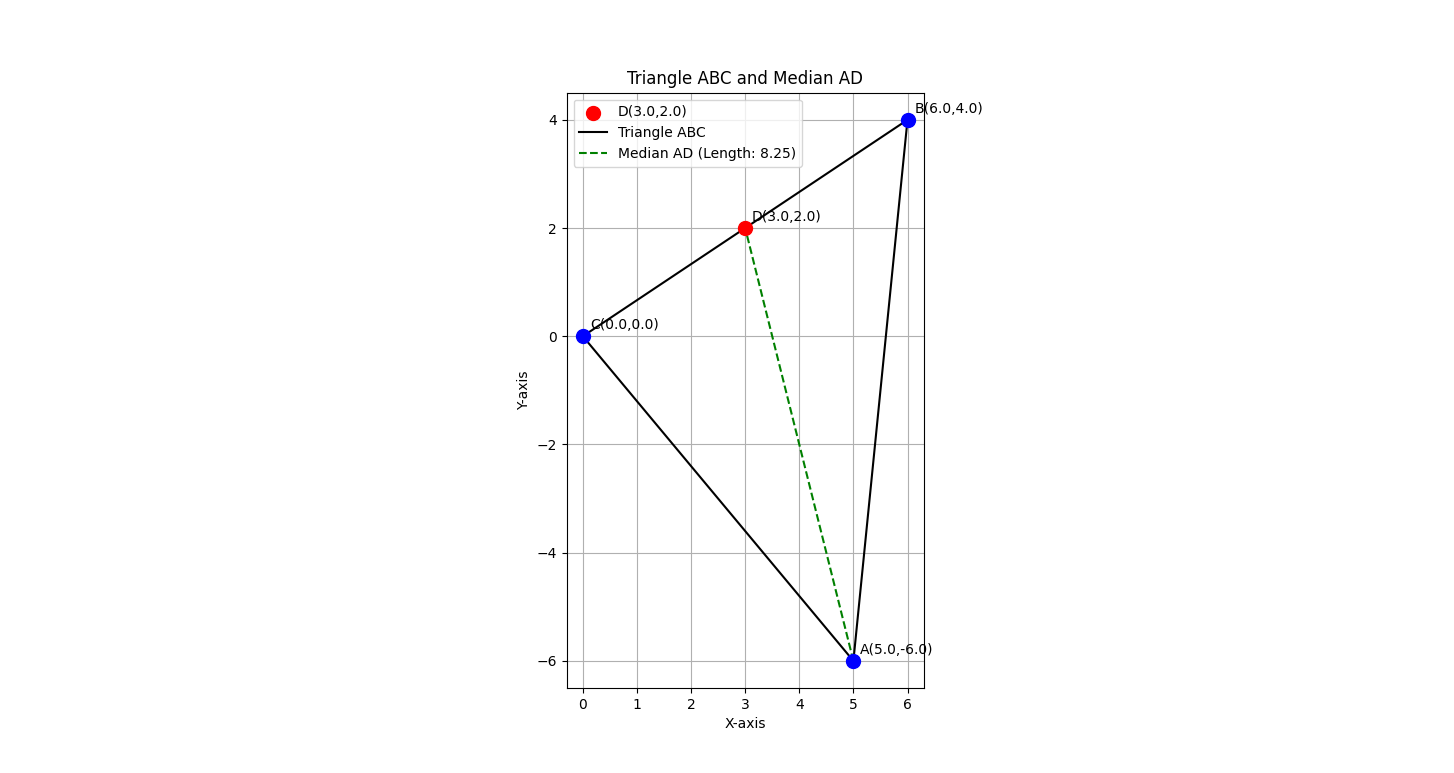
\includegraphics[width=1.0\columnwidth]{figs/fig1.png}
   \caption{}
   \label{fig:1}
\end{figure}


\end{document}
